\section{The Red Thread for this thesis}
\label{section_read_thread}
\textbf{\textit{NB}: Always connect software engineering, mobile analytics, and reliability.}
If every component in the system were reliable and complete we might not need or benefit from mobile analytics. Indeed they would be a distraction and wasteful. However, in the real-world every component be it software, service, system, person, or device has flaws and limitations. We are not omnipresent or omniscient - could mobile analytics provide remote insights into a small yet vital subset of software quality into helping development teams understand how their apps are performing in terms of their (un-) reliability? and can that information be used to help the developers address at least some of the underlying causes of the failures?

Information needs to flow from users' devices and reach the developers somehow in order for developers to understand the performance of their apps. Given the ongoing examples of misdeeds and corruptions in the application of data collected from user's activities and user's content - the dynamics of the information gathered, processed, and transferred in support of mobile analytics is also pertinent. 

Developer can plan for the future operations of the app in several ways, such as embedding code within an app to record events, context, and other data. They generally use an API to do so. They can also plan various processes, ~\emph{e.g.} their release, bug investigation, and triage processes. Others may choose not to plan ahead; As many have observed, including the business guru Peter Drucker,~\emph{Not making a decision is a decision}, as summed up in Truth 31 in the book by~\cite{gunther2013truth_about_better_decision_making}.

Implicit feedback mechanisms provided by various forms of usage analytics (mobile analytics) can improve developers' awareness of how the software is being used and how it is behaving. Some of these sources of feedback are instigated by developers using logging and/or mobile analytics APIs, others are instigated by library and/or platform providers. The feedback mechanisms are used to identify probable issues in mobile apps where the development team then choose to address at least a subset of those issues with the aim of improving the quality-in-use~\citep{} of future releases of that app. Of the various forms of mobile analytics this research concentrates on \textbf{platform-level analytics} together with \textbf{crash and error analytics}. It applies these forms of analytics with a focus on \textbf{stability} for Android apps available in Google Play Store.

The research is mainly empirical owing to the nature of usage analytics and the analytics tools which thrive on volume and realism. Mixed methods were used to expand the research, for instance by using static analysis into how developers use and maintain remote logging in the codebases of their Android apps. The case studies include examples where the researcher was:
\begin{enumerate}
    \item embedded: an active participant integrated into the project team,
    \item coach: of an existing team of developers who applied the concepts,
    \item interviewer: of various development teams to learn of their practices and results,
    \item analyst/observer: performing static analysis of opensource code repositories.
\end{enumerate}

The research includes several aspects seldom studied owing to the challenges of obtaining the case studies, for instance from behind the curtain in commercial projects with over a million users, and from sources again seldom visible to researchers \emph{i.e.} of mobile analytics for real-world mobile apps.

\newpage

\begin{figure}
    \centering
    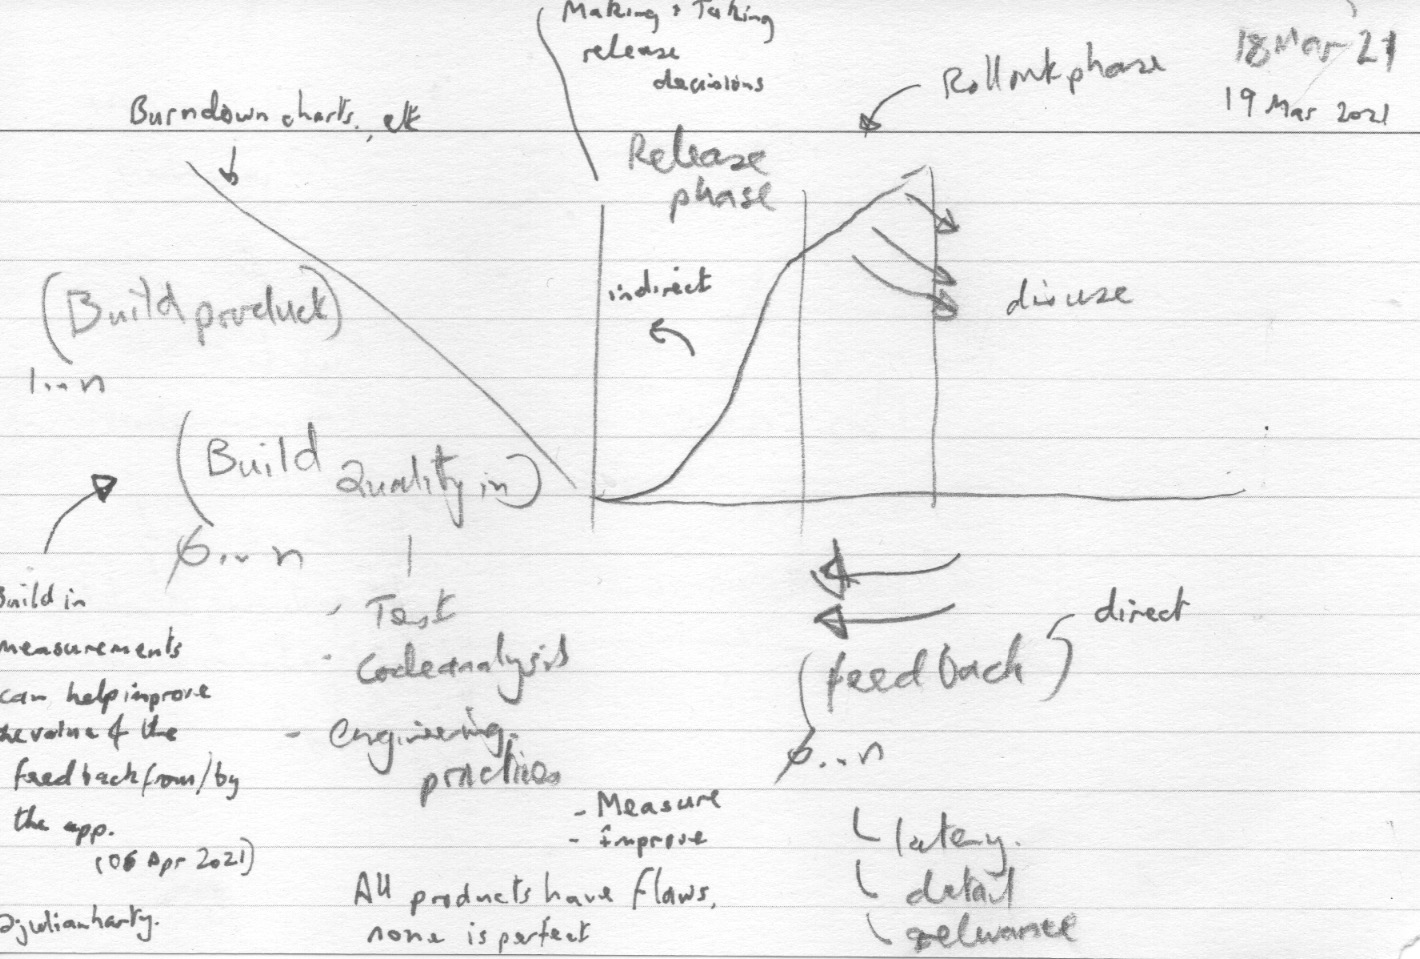
\includegraphics[width=15cm]{images/rough-sketches/Red-Thread-Rough-Sketch.jpeg}
    \caption{The lifecycle of a release and where mobile analytics provides feedback}
    \label{fig:red-thread-for-this-thesis}
\end{figure}

For any given release of a mobile app there are three phases:
\begin{enumerate}
    \item Building the product: which may incorporate practices and tools intended to ship a `quality product'. Some teams also incorporate logging and reporting to help measure the behaviours of the app in use, post release.
    \item The Release: For some projects this may be as simple as uploading a new binary and making it fully available. For others they may incorporate decisions and mechanisms to make each release with the aim of de-risking any undesirable/adverse effects of the new release.
    \item Live: where end users install and use the release of the app.
\end{enumerate}

Figure~\ref{fig:red-thread-for-this-thesis} illustrates these three phases together with some of the dynamics \emph{e.g.} of rollout and disuse of a release, and of feedback from whatever sources that the development teams can choose to pay attention to and apply.

Developers can choose when they will pay attention to the analytics; they can also choose the extent they wish to integrate analytics into their apps. Significant data is available for minimal effort, nonetheless the development teams who choose to invest in analytics are able to reap better and more relevant results. There are risks and responsibilities of the effects of collecting data and performing analysis on that data, practices outstrip legislation. It remains possible for sensitive findings to be discovered through the use of mobile analytics, nonetheless the ethical challenges are not unique to mobile analytics.

This research found that developers are able to materially improve the stability/reliability~\footnote{Stability is a term used by Google when they describe their Android Vitals service which is incorporated into Google Play Console. It includes measures of crashes and ANRs. An overview of Android Vitals is available online from various Google and Android sources including~\citep{android_vitals_overview_2019, android_vitals_best_practices}.}
%
of their mobile apps when they use the results of mobile analytics to assess the stability/reliability, identify groups of failures, triage the failures, and address the ones they decide to action. Where project teams stop paying attention to this process the failure rate increases of their new releases - the apps tend to entropy and failure.

Diligent developers and development teams can materially improve the stability/reliability of their apps through applying good coding, design and architecture patterns. Even these practices do not guarantee the releases will always be trouble-free. By paying ongoing attention to analytics during development, testing, and the rollout of releases flaws can be identified before the release reaches the majority of the userbase and teams can ameliorate the effects of many of the flaws.

\newpage 

\begin{figure}
    \centering
    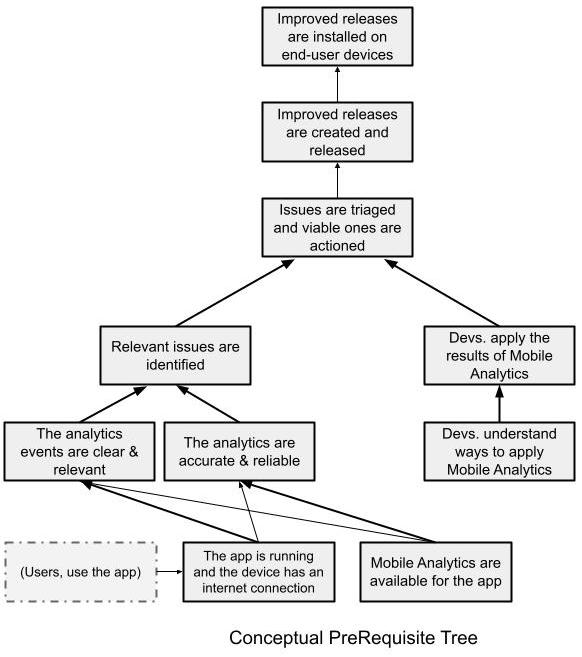
\includegraphics[width=12.5cm]{images/my/Conceptual_prereq_tree_Applying_Theory_of_Constraints_to_using_Mobile_Analytics_to_improve_Mobile_Apps.jpeg}
    \caption{Conceptual Prerequisites Tree: Using mobile analytics to improve mobile apps}
    \label{fig:using-toc-cpt-using-mobile-analytics-to-improve-mobile-apps}
\end{figure}

Figure~\ref{fig:using-toc-cpt-using-mobile-analytics-to-improve-mobile-apps} illustrates a conceptual prerequisite tree \footnote{(applying Theory of Constraints, see~\citep{goldratt2017_necessary_but_not_sufficient, lepore1999_deming_and_goldratt, scheinkopf1999_thinking_for_a_change})}. 
%
The underpinnings in terms of being able to improve mobile apps are threefold: 
\begin{enumerate}
    \item Users need to use the app. The app's behaviours will include errors and failures.
    \item The app needs connectivity together with at least one form of mobile analytics.
    \item Developers need to understand the outputs of mobile analytics and address pertinent issues in future releases of the app.
\end{enumerate}

Some issues can be ameliorated externally to the app, for instance though changes to servers that support API requests from apps, however many need changes to the app in order to be effective. 

If time-machines were available in software development developers might be able to go back in time and repair the current application on the user's mobile device. Conversely, a time-machine could enable users to return to the time and context when an event such as a failure occurred in order to help the developers understand contributory factors that led up to the failure and the aftermath. In 1999, time-machine computing was introduced as a way to help manage time in computing environments, for instance using a desktop environment - `TimeScape' - that supported time travelling on the computer, and time-casting to restore the application's context~\citep{rekimoto1999_time_machine_computing}. In mobile analytics, breadcrumbs~\citep{MacLean2015_pro_android_5_book} can be generated to help \emph{post-hoc} analysis of events that preceded a failure, and particularly crashes. 
%
For apps released as compiled binary files (the vast majority in iOS and Android app stores), improvements are generally made to a subsequent release than the one(s) where the failures have been occurring. And these subsequent releases need to be installed by the user population and used similarly in order to determine whether the improvements were worthwhile. Some users keep older releases and others stop using the app. 


% [4] Joorabchi, Mona Erfani, Ali Mesbah, and Philippe Kruchten. "Real challenges in mobile app development." Empirical Software Engineering and Measurement, 2013 ACM/IEEE International Symposium on 10 Oct. 2013: 15-24.


Many developers fail to address all the issues identified through use of mobile analytics and a key influence is their perceived ability to successfully address issues identified by the analytics. Furthermore, these issues are collectively only one of many demands for their time and attention. Human, organisational, and business factors all influence the extent mobile analytics is a) used and b) the results addressed. This research touches on both the mechanics of applying mobile analytics together with the `game' which are the higher-level human nature aspects which affect the application and the value of applying the mechanics. Figure~\ref{fig:the-mechanics-the-game} provides a simple illustration of the game and the mechanics.

\begin{figure}
    \centering
    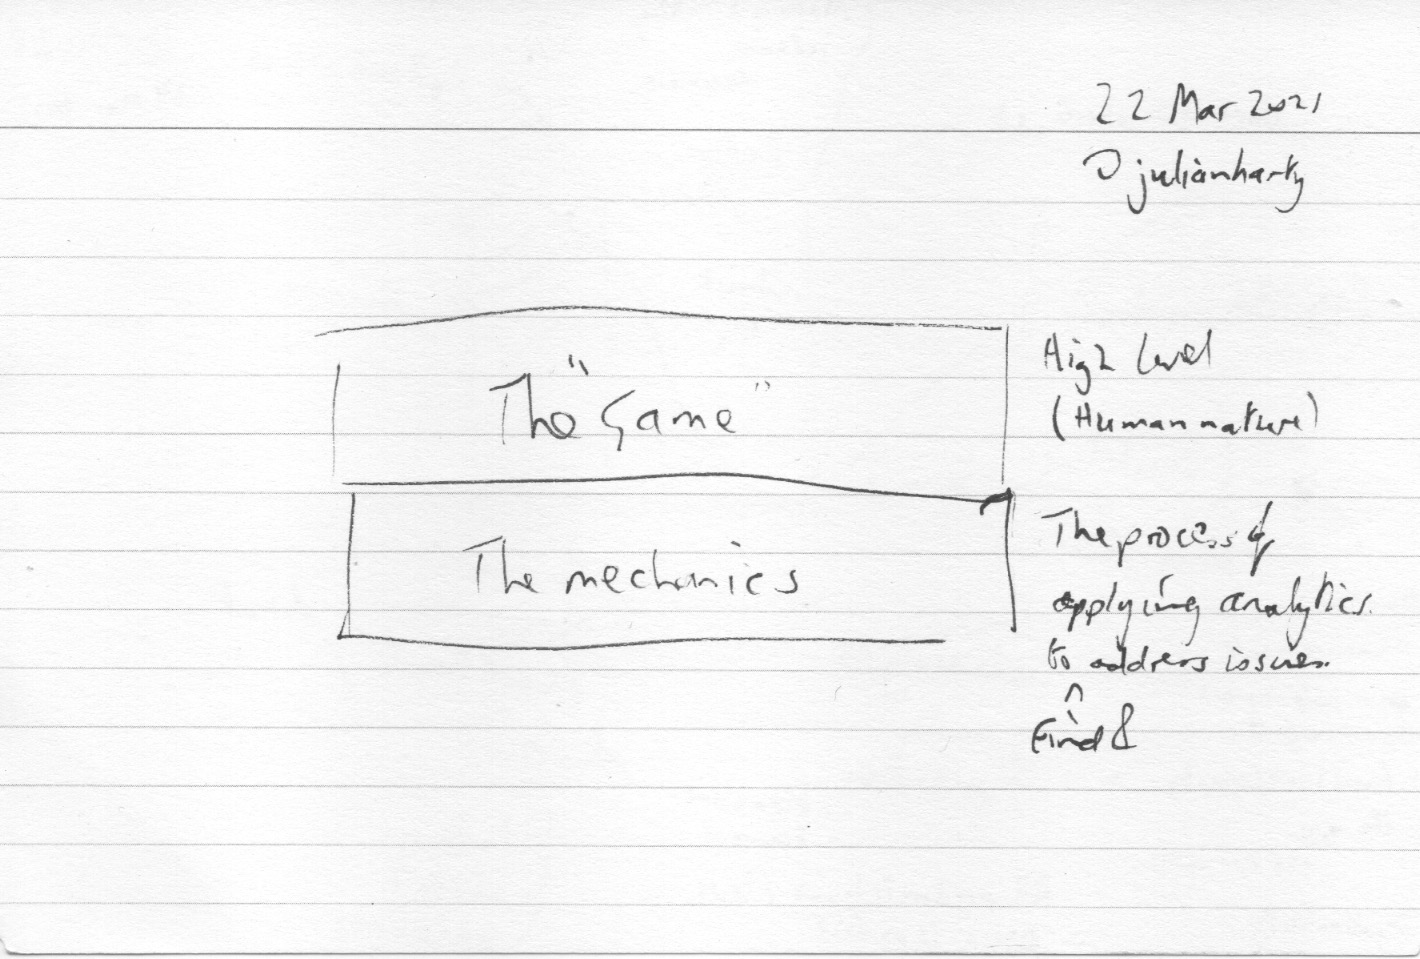
\includegraphics[width=15cm]{images/rough-sketches/The-Mechanics-The-Game.jpeg}
    \caption{The Mechanics and The Game of using Mobile Analytics}
    \label{fig:the-mechanics-the-game}
\end{figure}

Analytics providers have a major influence on the efficacy of the application of mobile analytics. There are limitations and flaws in the various tools this research has encountered regardless of their source (\emph{e.g.} in-house proprietary, opensource, free and paid-for commercial proprietary offerings). Nonetheless, flawed offerings are still able to be used to deliver improvements in the mobile apps. Specialised startups such as Iteratively aim to increase the coherence of embedded analytics (those embedded into the apps) while also increasing compliance. HP's AppPulse Mobile provided no-code analytics for mobile apps where their tools automatically instrumented the binary to add the analytics; several providers offered GUI interaction recording and `heatmaps' generated using aggregated recordings of touch screen interactions.

Those who applied the results of mobile analytics were able to increase the stability/reliability of their mobile apps. The amounts of improvements varied based on various factors such as:
\begin{itemize}
    \item The starting point for the app.
    \item The amount of ongoing engagement of the development team.
    \item The choices of mobile analytics services and the use of proactive event recording using the related analytics libraries.
    \item The sources and causes of some of the issues being reported - some where far harder to diagnose than others, and several originated outside the actually codebase of the mobile app where it might be impractical to truly fix the source of the issue.
\end{itemize}

\noindent
\rule{\textwidth}{0.4pt}

The case studies illustrate manifold facets of applying (and ignoring) mobile analytics across various contexts of engagement, across various types of app, and from several perspectives including the organizations who create the mobile analytics.